\chapter{Markup}
A manuscript can be a seamless current of words and still make perfect sense to
an author. To truly capture its meaning in a clear and unambiguous manner,
however, the author will often need to supplement the manuscript with a set of
annotations. At a more fundamental level, this refers to the compliance with the
orthographic rules---such as the correct spelling, capitalization, word breaks,
and punctuation---that are specific to the language of the document. It is not
at all unreasonable to expect that this basic compliance should be already met
by the manuscript. At a higher level, this consists of discovering and marking
up the inner order and logic of the text, so that the resulting document can
later be typeset in a way that visually reflects its structure.

It is not unusual for an author to write and mark up their manuscript at the
same time. Nevertheless, each of the two activities represents a distinct
concept. Writing is the process of breaking ideas down into raw sequences of
words. To mark up these words then is to take and reassemble them back into
meaningful units of linguistic thought.

\index{markup!logical}\index{markup!presentation}
Markup can be created using a variety of \termpl*{markup language}. Aside from
\term*{logical markup}, which captures the logical structure of a document,
markup languages may also provide \term*{presentation markup}, which directly
impacts the visual properties of the document but carries no semantic
information. The usage of presentation markup makes it impossible to separate
the markup from the design and to capture the structure of the document. As a
result, the consistency in the design of each logical part of the document needs
to be ensured manually, and future changes of design become error-prone and
tedious. In this regard, logical markup is to design what style guides are to
writing: a means of ensuring internal consistency that should be used whenever
possible.

\section{Meta Markup Languages}
\subsection{The General Markup Language}
The situation engulfing digital typesetting was growing increasingly frustrating
for publishers in the 1960s. The markup languages used by different typesetting
systems varied wildly and once a publisher had a large collection of documents
typeset via a given company, switching to another one could be a costly
venture. This power imbalance artificially increased the price of digital
typesetting, leading to a demand for a universal markup language.

This demand was met by a project developed\sidenote{
  More information about the project can be found within
  \citework{goldfarb96} and \citework*(SGML: The Reason Why and the First
  Published Hint)[]{goldfarb97:whySGML}.
} at the Cambridge Scientific Center of \acronym{IBM} in the early 1970s. The
project aimed at imbuing a text editor with the ability to query, edit, and
display documents from a central repository to allow the usage of computers in
legal practice. Very early on in the development it became apparent that the
main problem were going to be the markup languages in which the documents were
written. These languages varied wildly and many of them comprised largely
presentation markup, which made information retrieval impossible without heavy
use of heuristics. To resolve these issues, a unifying markup language called
\acronym{GML} was drafted. The language was released~\cite{goldfarb81} to the
public in \citeyear{goldfarb81} and finally standardized in \citeyear{iso86} as
\acronym{SGML}\sidenote{
  The authoritative resource on \acronym{SGML} is \citework{goldfarb91}, which
  includes the full text of the standard bearing extensive annotations.
}.~\cite{iso86}

\Acronym{SGML} documents consist of text mixed with \termpl*{tag}%
\acroindex[!tag]{SGML}, which delimit meaningful sections of the document called
\termpl*{element}\acroindex[!element]{SGML}. Elements may carry additional
information in \termpl*{attribute}\acroindex[!attribute]{SGML}. Additionally,
\acronym{SGML} documents may contain miscellaneous instructions for the programs
that are processing them as well as human-readable comments. An umbrella term for
the various parts of \acroshort{SGML} document is
\termpl*{node}\acroindex[!node]{SGML}. Repeated strings of text can be declared
as \termpl*[entities]{entity} \acroindex[!entity]{SGML} that can be used
throughout the document in place of the original strings. 

Although the described structure is shared by all \acronym{SGML} documents, the
actual syntax, as well as the restrictions regarding the contents and the
attributes of individual elements, are declared within a \acronym{DTD}, which
can be different for each document. It is worth noting that a \acronym{DTD} only
declares the syntax of an \acroshort{SGML} document; the semantics of the
individual elements and their attributes are left to the interpretation of the
program processing the document. The syntax and the constraints imposed by a
\acronym{DTD} define an \term*{application of \acronym{SGML}}%
\acroindex[!application]{SGML}. An \acronym{SGML} document is considered to be a
valid instance of an \acroshort{SGML} application, when it conforms to the
corresponding \acronym{DTD}.

\subsection{The Extensible Markup Language}
Although \acronym{SGML} was designed to be the general format for data exchange,
the complexity of the specification and the lack of support for Unicode (see
Section~\ref{sec:ucs+unicode}) proved to be a major hindrance preventing its
wider adoption and the development of \acroshort{SGML} tools. In a response,
\acronym{W3C} published a specification of \acronym{XML} in \citeyear{bray98}.
Along with the introduction of \acronym{XML}, the \acroshort{SGML} specification
received a technical corrigendum~\cite{goldfarb97:webSGML}, which turned
\acronym{XML} into an \acronym{SGML} application defined through a
\acronym{DTD}.

\begin{figure}
  \inputcode[xml]{examples/02/recipe.xml}
  \caption{An example \acronym{XML} document\filenamecap{recipe.xml}}
  \label{fig:recipe}\bigskip
\end{figure}

\begin{figure}
  \fsidenote{\acronym{DTD}s in \acronym{SGML} and \acronym{XML} documents can be
    either linked to the document through \code[dtd]{PUBLIC} and
    \code[dtd]{SYSTEM} identifiers (top), directly embedded in the document
    (middle), linked to the document and then extended by an embedded
    specification (bottom), or omitted.}
  \inputcode[dtd]{examples/02/dtdtypes}
  \caption{An example \acronym{DTD}}
  \label{fig:recipe-dtd}
\end{figure}
        
\begin{figure}
  \inputcode{examples/02/recipe.rnc}
  \caption{A reformulation of the \acronym{DTD} from Figure \ref{fig:recipe-dtd}
    in the compact syntax of the \acronym{Relax NG} schema
    language\filenamecap{recipe.rnc}. Note how \acronym{Relax NG} allows us to
    constrain the attribute data types.}
  \label{fig:recipe-rnc}
\end{figure}

This \acronym{DTD} completely fixes the syntax of \acronym{XML} documents, which
makes it possible to differentiate between two levels of correctness. An
\acronym{XML} document is considered to be \term*{well-formed}%
\acroindex[!well-formedness]{XML}, when it conforms to the \acronym{DTD} that
specifies the syntax of \acronym{XML} and to the \acroshort{XML} specification.
An \acroshort{XML} document is considered to be
\term*{valid}\acroindex[!validity]{XML} against an \acronym{DTD}, when it is
well-formed and conforms to the said \acronym{DTD}. Along with \acronym{DTD}s,
there exists a wealth of \termpl*{schema language}\acroindex[!schema
language]{XML}\sidenote{
  A list of tools for the manipulation of files in \acronym{XML} schema
  languages is maintained on the Web site of \acronym{W3C} at
  \url{http://www.w3.org/XML/Schema}.
} for \acronym{XML}---such as \acroshort{W3C} \acroshort{XML} Schema%
\acroindex[!Schema]{XML}, \acronym{Relax NG}, or Schematron---that can be used
to check the validity of an \acroshort{XML} document instead of a \acronym{DTD}.
The constrains imposed by either a \acronym{DTD} or a schema define an
\term*{application of \acronym{XML}} (also \term*{language} or \term*{format}).
\acroindex[!application]{XML} \acroindex[!language]{XML}
\acroindex[!format]{XML}

\begin{figure}
  \inputcode[xml]{examples/02/recipe.xsd}
  \caption{A reformulation of the \acronym{DTD} from Figure \ref{fig:recipe-dtd}
    in the \acroshort{XML} Schema \acroindex[!Schema]{XML}
    language\filenamecap{recipe.xsd}}
  \label{fig:recipe-xsd}
\end{figure}

\begin{figure}
  \inputcode[sh]{examples/02/recipe.sh}
  \caption{\acronym{XML} documents can be easily validated against \acronym{XML}
    schemata using the free command-line program of \cliutil{xmllint}.}
\end{figure}

Along with schema languages, other supplementary languages exist, such as
\inx{XPointer}, \inx{XPath}, and \inx{XQuery} for the retrieval of data from XML
documents, \acronym{CSS} for the specification of \acroshort{XML} document
design, and the various languages for the description of Web resources that we
will discuss in Section~\ref{sec:semantic-web}.

\begin{figure}[!b]
  {\tikzstyle{level 1}=[sibling distance=\baselineskip, level distance=1.5cm]
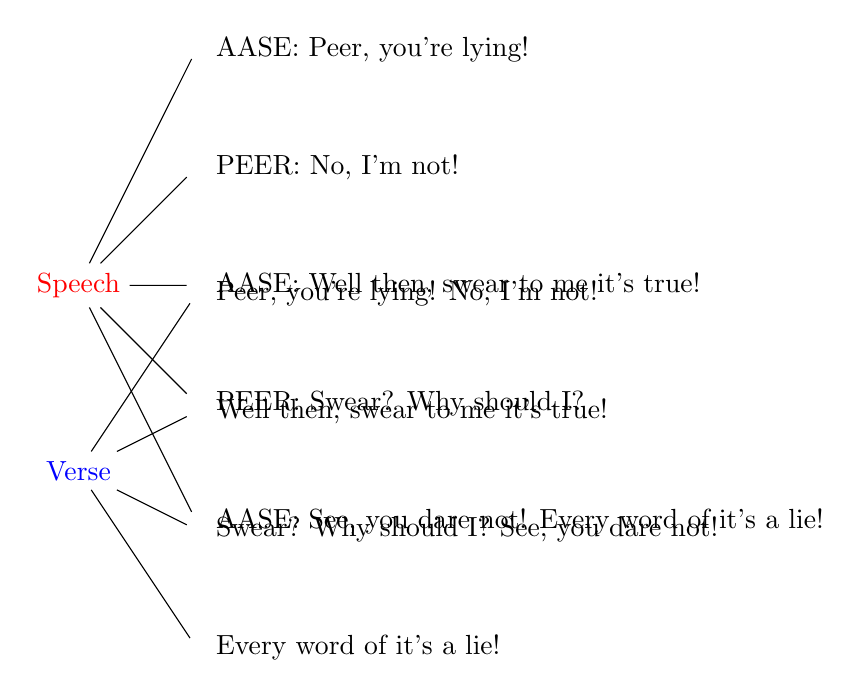
\begin{tikzpicture}[grow=right]
  \node {\textcolor{red}{Speech}}
    child {
      node [label=right:{AASE: See, you dare not! Every word of it's a
        lie!} ] {}}
    child {
      node[label=right:{PEER: Swear? Why should I?}] {} }
    child {
      node[label=right:{AASE: Well then, swear to me it's true!}] {}}
    child {
      node[label=right:{PEER: No, I'm not!}] {} }
    child {
      node[label=right:{AASE: Peer, you're lying!}] {} };
  \node [below=5\baselineskip] {\textcolor{blue}{Verse}}
    child {
      node[label=right:{Every word of it's a lie!} ] {}}
    child {
      node[label=right:{Swear? Why should I? See, you dare not!}] {} }
    child {
      node[label=right:{Well then, swear to me it's true!}] {}}
    child {
      node[label=right:{Peer, you're lying! No, I'm not!}] {} };
\end{tikzpicture}}%
\begin{Verbatim}[commandchars=\\\{\},codes={\catcode`$=3\catcode`^=7\catcode`_=8}]
<(\textcolor{blue}{V})line>
  <(\textcolor{red}{S})speech who="Aase">Peer, you're lying!</(\textcolor{red}{S})speech>
  <(\textcolor{red}{S})speech who="Peer">No, I'm not!</(\textcolor{red}{S})speech>
</(\textcolor{blue}{V})line><(\textcolor{blue}{V})line>
  <(\textcolor{red}{S})speech who="Aase">Well then,
    swear to me it's true!</(\textcolor{red}{S})speech>
</(\textcolor{blue}{V})line><(\textcolor{blue}{V})line>
  <(\textcolor{red}{S})speech who="Peer">Swear, why should I?</(\textcolor{red}{S})speech>
  <(\textcolor{red}{S})speech who="Aase">See, you dare not!
</(\textcolor{blue}{V})line><(\textcolor{blue}{V})line>
  Every word of it's a lie!</(\textcolor{red}{S})speech>
</(\textcolor{blue}{V})line>
\end{Verbatim}
%
  \caption{The markup of the dramatic and metrical views of \person{Henrik
    Ibsen}'s \work{Peer Gynt} using the \identifier{CONCUR} feature of
    \acronym{SGML}. This figure was inspired by the figures found in the article
    \protect\citework{sperberg04}.}
\end{figure}

A notable feature of \acronym{XML} unavailable in \acronym{SGML} are
\termpl*{namespace}\acroindex[!namespace]{XML}, which were added to the
\acroshort{XML} specification~\cite{bray99} in \citeyear{bray99}. Namespaces
enable the inclusion of elements and attributes from different \acronym{XML}
applications within a single \acronym{XML} document; each application is
uniquely identified through an \acropl{IRI}. Namespaces in \acronym{XML} are a
spiritual successor of a more expressive \acronym{SGML} feature of
\identifier{CONCUR}\index{CONCUR@\identifier{CONCUR}}, which makes it possible
to mark up several structural views of a single document. Unlike with
\identifier{CONCUR}, which ties each view to an \acroshort{SGML} \acronym{DTD},
there exists no general mechanism for the translation of the \acropl{IRI} to
\acronym{XML} schemata. This makes it impossible to validate namespaced
\acronym{XML} documents, unless all the \acropl{IRI} and their schemata are
known to the parser.

%%% Živoucí CONCAT <http://webylon.info/K.24>
%%% Popis SGML deklarace pro ISO/IEC15445
%%%   <http://www.angelovic.cz/internet/sgml-deklarace.html#concur>

Due to the reduced complexity of \acronym{XML} compared to \acronym{SGML}, the
language was adopted by the industry and has superseded \acronym{SGML} in most
applications. Some of the applications of \acronym{XML} for document preparation
include DocBook\acroindex[!DocBook]{XML}\sidenote{
  The authoritative resource on the DocBook \acronym{XML} format is
  \citework{walsh10}. The book itself is written in DocBook and its source code
  is publicly available at \url{http://docbook.org}.
}---a technical documentation markup language used for authoring books by
publishers such as O'Reilly Media and for documenting software at companies such
as Red Hat, \acroflat{SuSE}, or Sun Microsystems---, \acronym{TEI}---a general
text encoding markup language for the use in the academic field of digital
humanities---, \acronym{MathML}---a markup language for the description of
mathematical formulae---, or \acronym{SVG}---a vector graphics format. Other
\acroshort{XML} applications, such as \acroshort{XHTML} and
\acroshort{RDF}/\acroshort{XML}, will be discussed in
Section~\ref{sec:www-markup}.
      
\section{Markup on the World Wide Web}\label{sec:www-markup}
\subsection{The Hypertext Markup Language}
In \citeyear{bernerslee89}, an English computer scientist named \person{Timothy
John Berners-Lee} proposed a decentralized system for sharing documents within
\acronym{CERN}~\cite{bernerslee89}. The system laid foundation for the Web and
earned its author knighthood. The markup language used to write documents for
the system was an application of \acronym{SGML} called \acronym{HTML}. In 1993,
the Web started to gain traction among the general public owing largely to the
release of the first graphical Web browser Mosaic, which paved way for the Web
browsers of today. In 1994, \person{Timothy John Berners-Lee} formed
\acronym{W3C}, which has since developed the standards for the Web.

The first standard version of \acronym{HTML} was \acronym{HTML} 2.0
\cite{bernerslee95} published in \citeyear{bernerslee95}. As the Web was
becoming ubiquitous, it began accumulating an increasing number of documents
that weren't valid instances of \acronym{HTML}, since most Web browsers faced
with a malformed document would act in accordance with the Postel's law%
\sidenote{
  The Postel's law states that one should be conservative in what they send, but
  liberal in what they accept.~\cite[sec.\,2.10]{postel80} It is one of the base
  principles for building robust communication protocols.}
and try to render the document despite its deficiencies. In an attempt to unify
the way malformed \acronym{HTML} documents were rendered across the Web
browsers, \acronym{W3C} acknowledged and documented this behavior as a part of
the \acroshort{HTML}5 specification~\cite[sec.\,8.2]{hickson14}. An example of
a non-conforming \acroshort{HTML}5 document and its canonical interpretation is
given in Figure \ref{fig:overlapping-elements}.

\begin{figure}[b]
  \inputcode[html]{examples/02/malformed.html}
  \caption{The first line contains overlapping elements and, as such, can't be a
    part of a valid \acronym{HTML} document. Nevertheless, browsers should
    handle it identically to the second line.}
  \label{fig:overlapping-elements}
\end{figure}

Initially, \acronym{HTML} only comprised a mixture of
logical\index{markup!logical} and presentation markup\index{markup!presentation}
with fixed visual interpretation. This changed with the specification of
\acronym{CSS}, which was introduced by \acronym{W3C} in \citeyear{lie96}. The
language enabled the specification of the visual properties for any
\acroshort{HTML} element, which enabled the separation of document markup and
design, effectively eliminating the need for the presentation markup.

\begin{figure}
  \inputcode[html]{examples/02/presentation-markup.html}%
  \separatorcaption{An excerpt from the Web site of the \acroshort{CSS} Zen
    Zarden located at \protect\url{http://csszengarden.com}. The document above
    was created using the \acroshort{HTML} presentation
    markup\index{markup!presentation}. The document below achieves the same
    appearance by the combination of logical markup\index{markup!logical} and
    \acronym{CSS}.}
  \inputcode[html]{examples/02/logical-markup.html}
\end{figure}

During the same period, an initial version of a scripting language called
\inx{JavaScript}~\cite{ecma97} was drafted and incorporated into Netscape
Navigator 2.0\sidenote{
  \inx{JScript} and \inx{VBScript} competed directly with JavaScript, but they
  never saw implementation outside Microsoft browsers.
}---one of the contemporary leading web browsers and a descendant of the
original Mosaic browser. As a part of a joint effort by Sun Microsystems and
Netscape Communications to bring the programming language of Java into web
browsers, JavaScript was supposed to complement Java
applets~\cite{netscape95}---a role it has since outgrown. Standardized in
\citeyear{ecma97}~\cite{ecma97}, JavaScript blurred the line between static
documents and interactive applications and remains the predominant client-side
programming language of the Web. However, since the support of JavaScript by a
Web browser is fully optional, it is considered a good practice not to depend on
JavaScript for the rendering of \acroshort{HTML} documents. In the case of
interactive \acroshort{HTML} applications, this recommendation may be relaxed.

\subsection{The Extensible Hypertext Markup Language}
Ever since the release of \acronym{XML} in 1998, \acronym{W3C} entertained the
idea of turning \acronym{HTML} into an application of \acronym{XML}, rather than
of \acronym{SGML}, as exemplified by the working draft of \citework{raggett98}.
Unlike \acronym{HTML} parsers, whose acceptance of malformed content makes them
complex, \acronym{XML} parsers are required to strictly refuse \acronym{XML}
documents that aren't well-formed~\cite[Section~1.2, Terminology]{bray98},
leading to architectural simplicity and decreased computational requirements. As
a result, reformulating \acronym{HTML} in \acronym{XML} was suggested as a way
to bring the Web to mobile, embedded, and other devices limited in their
computational resources and to reduce the amount of malformed documents on the
Web in general. Other perceived advantages included the ability to use
\acronym{XML} tools for web documents and to include instances of other
\acronym{XML} applications---such as \acronym{MathML} and
\acronym{SVG}---directly into web documents through \acronym{XML} namespaces.

The idea was brought to fruition in the \acronym{XML} application of
\acronym{XHTML}. However, the supposed benefits proved to be too marginal to
warrant migration from \acronym{HTML}. The speed advantages of the simplified
processing were largely offset by the lack of support for incremental rendering,
since it is impossible to validate and render partially downloaded
\acroshort{XHTML} documents and the advances in the area of mobile devices made
\acronym{HTML} processing sufficiently fast. The lack of ways to provide
alternative content for browsers that would not support the \acroshort{XML}
applications instantiated in the \acroshort{XHTML} documents also reduced the
usefulness of the \acroshort{XML} namespaces in \acronym{XHTML} considerably. As
a result, \acronym{XHTML} has yet to succeed in replacing \acronym{HTML} and
remains a minority markup language on the Web.

%%% Content-Negotiation Techniques to serve XHTML as text/html and
%%% application/xhtml+xml
%%%   <http://www.w3.org/2003/01/xhtml-mimetype/content-negotiation>

\subsection{The Semantic Web and Linked Data}\label{sec:semantic-web}
The Web is based on the idea of a distributed and globally available network of
human knowledge. The languages of \acronym{HTML}, \acronym{XHTML}, \acronym{CSS}
and JavaScript form the foundation of the human-readable parts of the Web, but
are inadequate for creating a network of machine-readable data that could be
navigated by software agents.\sidenote{
  The idea of a network of machine-readable data was described by
  \person{Tim Berners-Lee} in \citeyear{bernerslee06} in the article
  \citework{bernerslee06}.}
Drawing from the research in the field of knowledge representation,
\acronym{W3C} created \acronym{RDF} in \citeyear{lassira99}---a language for the
description of resources on the Web.

An \acroshort{RDF} document represents data as a set of \termpl*{triplet}%
\acroindex[!triplet]{RDF}. Each triplet comprises a
\term*{predicate}\acroindex[!predicate]{RDF}, a \term*{subject}%
\acroindex[!subject]{RDF}, and an \term*{object}\acroindex[!object]{RDF},
where both the predicate and the subject are specified as \termpl*{resource}
\acroindex[!resource]{RDF} using \acropl{IRI}. If the object of a triplet
$(p,s,o)$ is also a resource, the triplet can be interpreted as a subject $s$
being in a relation $p$ with the object $o$. If the object is a \term*{literal
value} \acroindex[!literal]{RDF} rather than a resource, the triplet can be
interpreted as a subject $s$ having a property $p$ with the value $o$.

Resources in \acronym{RDF} are specified via \acropl{IRI} to prevent naming
collisions in \acronym{RDF} documents created independently by distinct authors.
These \acropl{IRI} do not need to point to any existing web page, and---beside
the small set of standard resources specified within the \acroshort{RDF}
specification---they carry no inherent meaning. In order to describe a set of
resources, the relationships between them, and their intended meaning in an
\acroshort{RDF} document, an extension of the set of standard resources called
\acroshort{RDF} Schema~\cite{brickley04} can be used. The resulting documents
are called \termpl*[ontologies]{ontology} \acroindex[!ontology]{RDF} and can be
used for automated reasoning about \acronym{RDF} documents containing resources
described by the ontology.\sidenote{
  A list of ontologies that are fully documented, honor the current best
  practices, and are supported by various tools can be found on the
  \acroshort{W3C} wiki at \url{http://www.w3.org/wiki/Good_Ontologies}.
} Some of the well-known ontologies include \acronym{DC}---an ontology for the
generic description of resources, both digital and physical---,
\acronym{FOAF}---an ontology for the description of people and their social
relationships---, or the Music Ontology---an ontology for the description of
entities related to the music industry, such as albums, artists, tracks, and
events. More expressive standards for the creation of ontologies, such as
\acronym{OWL}, also exist.

\acronym{RDF} documents can be represented through many languages, including
\acroshort{XML}~\cite{lassira99}, \acronym{JSON-LD},
\inx{Turtle}~\cite{beckett14:turtle}, and \inx{N-Triples}~\cite{beckett14:nt}.
Although \acroshort{RDF} documents in any of these representations can be
included in or linked to \acroshort{HTML} and \acroshort{XHTML} documents, this
will often result in the undesirable duplication of data. To prevent this, the
language of \acronym{RDFa} makes it possible to mark parts of the
\acroshort{HTML} or \acroshort{XHTML} document as \acronym{RDF} data. The usage
of \acronym{RDF} in conjunction with \acronym{HTML} and \acronym{XHTML} is
intended to gradually obsolete the loosely-defined use of \acroshort{HTML} and
\acroshort{XHTML} attributes, the \element{meta} and \element{link} elements,
and the \acronym{CSS} class names to include additional machine-readable metadata
into the documents on the Web---a technique known as \term{microformatting}.

\begin{figure}
  \inputcode[xml]{examples/02/john.rd}\vspace{-.4em}%
  \inputcode{examples/02/john.nt}\vspace{-.4em}%
  \inputcode{examples/02/john.ttl}
  \caption{An example \acronym{RDF} document using
    the \acronym{DC} and \acronym{FOAF} ontologies in the languages of
    \acronym{RDF}/\acronym{XML}\filenamecap[top]{john.rd},
    \inx{N-Triples}\filenamecap[middle]{john.nt}, and
    \inx{Turtle}\filenamecap[bottom]{john.ttl}}\label{fig:rdf-doc}
\end{figure}

\begin{figure}
  \inputcode[html]{examples/02/john.html.linked-rdf}
  \separatorcaption{Above is an \acroshort{HTML} document linked to the
    \acroshort{RDF} document from Figure \ref{fig:rdf-doc}. Below is the same
    \acroshort{HTML} document with the \acroshort{RDF} data directly embedded
    using the \acroshort{RDFa} language.}
  \inputcode[html]{examples/02/john.html.rdfa}
\end{figure}

\begin{figure}
  {\tikzstyle{level 1}=[sibling distance=6\baselineskip, level distance=0.5cm]
\tikzstyle{level 2}=[sibling distance=6\baselineskip, level distance=0.5cm]
\centerline{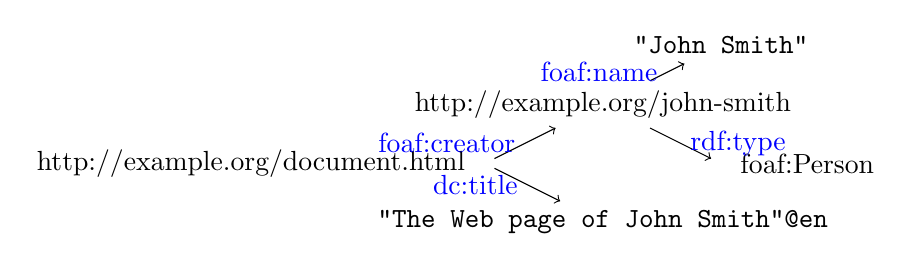
\begin{tikzpicture}[grow=right,->]
  \node[label=left:{\url{http://example.org/document.html}}] {}
    child { node {\texttt{"The Web page of John Smith"@en}}
      edge from parent
      node[left] {\textcolor{blue}{dc:title}}}
    child { node {\url{http://example.org/john-smith}}
      child { node[label=right:{foaf:Person}] {}
        edge from parent
        node[right,align=left] {\textcolor{blue}{rdf:type}}}
      child { node {\texttt{"John Smith"}}
        edge from parent
        node[left] {\textcolor{blue}{foaf:name}}}
      edge from parent
      node[left] {\textcolor{blue}{foaf:creator}};
    };
\end{tikzpicture}}}

  \caption{A graph of the \acroshort{RDF} document in Figure \ref{fig:rdf-doc}}
\end{figure}

%%% Linked Data
%%%   <http://www.w3.org/DesignIssues/LinkedData.html>
%%%
%%% Tim Berners-Lee: The next web
%%%   <http://www.ted.com/talks/tim_berners_lee_on_the_next_web>
%%%
%%% The SPARQL Query Language for RDF (SPARQL) and the (at the time of
%%% writing only drafted) Linked Data Fragments RDF query interfaces
%%%   <http://www.w3.org/TR/rdf-sparql-query/>
%%%   <http://linkeddatafragments.org/specification/>
%%%
%%% The Rule Interchange Format (RIF)
%%%   <http://www.w3.org/TR/rif-overview/>
        
\section{Document Preparation Systems}
Some of the existing markup languages are tied directly to specific
\acropl{DPS}. These \acropl{DPS} can be categorized into the
\term*{batch-oriented}\acroindex[!batch-oriented]{DPS}, which process text files
into printable output documents on demand, and the
\term*{interactive}\acroindex[!interactive]{DPS} (also \acronym{WYSIWYG}), which
allow the user to directly edit an approximation of the output document through
a visual editor. The price for the mild learning curve of interactive
\acropl{DPS} are the more primitive typesetting algorithms, which need to be
sufficiently fast to enable real-time user interaction, and the reduced
flexibility stemming from the usage of a \acronym{GUI}, which, although often
intuitive for simple tasks, seldom matches the power of the markup languages
used by batch-oriented \acropl{DPS}.

\subsection{Batch-oriented Systems}
One of the archetypal batch-oriented \acropl{DPS} are \cliutil*{troff}%
\index{troff@\cliutil*{troff}}, whose function is to produce output for general
printers, and \cliutil*{nroff}%
\index[see{\cliutil*{troff}}]{nroff@\cliutil*{nroff}}, whose function is to
produce output for line printers and text terminals. Both are proprietary
software developed for the Unix operating system at the beginning of 1970s by
\acronym{ATnT}. An alternative to \cliutil*{nroff} and \cliutil*{troff} is
\cliutil*{groff}\index[see{\cliutil*{troff}}]{groff@\cliutil*{groff}}, which was
developed as free software for the \acronym{GNU} project in 1980 by the members
of the \acronym{FSM}. \Cliutil*{groff} combines the capabilities of both systems
and is used extensively for the markup of documentation in \Unices. The
markup language of \cliutil*{groff} combines presentation
markup\index{markup!presentation} with programming constructs and enables the
definition of logical markup\index{markup!logical} through user macros. The
standard macro packages for \cliutil*{groff} include \identifier{man} for the
\index{troff@\cliutil*{troff}!\identifier{man}} formatting of documentation,
\identifier{me} \index{troff@\cliutil*{troff}!\identifier{me}} for the creation
of research papers, and the more recent \identifier{mom}
\index{troff@\cliutil*{troff}!\identifier{mom}} for general typesetting tasks.
Special markup invokes preprocessors that can be used for the typesetting of
tables, equations, and vector graphics.

\begin{figure}
  \vspace{.45em}%
  \fbox{\includegraphics[clip,trim=1.7cm 12.6cm 1.7cm 1.3cm,%
    width=0.975\textwidth]{examples/02/poe-groff.pdf}}%
  \vspace{.45em}%
  \inputcode[groff]{examples/02/poe.groff}
  \caption{An excerpt from the beginning of \person{Edgar Allen Poe}'s
    \work*{Cask of Amontillado}\workindex{the Cask of Amontillado} as a
    text marked up using the \identifier{mom} macro package of \cliutil*{groff}
    (below) and the output document (above). The marked up text was borrowed
    from the web page of \identifier{mom}~\cite{schaffter15}.}
  \label{fig:poe}
\end{figure}

%%% The Groff and Friends HOWTO
%%%   <http://troff.org/TheGroffFriendsHowto.pdf>
%%%
%%% Writing Macros
%%%   <https://www.gnu.org/software/groff/manual/html_node/Writing-Macros.html>
%%%
%%% A User's Guide to the Lout Document Formatting System
%%%   <https://www.urz.uni-heidelberg.de/imperia/md/content/urz/programme/text/lout.pdf>

Another notable free batch-oriented \acronym{DPS} is
\TeX\index{TeX@\TeX}\sidenote{
  The circumstances that led to the creation of \TeX\ and the surrounding tools
  are thoroughly documented in \citework{knuth98}.
}, which was developed in the 1970s by an American professor of computer science
\person{Donald Knuth} after he had received galley proofs for the second volume
of his monograph, \work{the Art of Computer Programming}, and found the
appearance of mathematical formulae distasteful. As a result, the typesetting of
mathematics is a central theme in \TeX, rather than an afterthought, which
differentiates it from most other \acropl{DPS} and which contributes to the
massive popularity \TeX\ has enjoyed among academics. Much like in the case of
\cliutil*{troff} and its derivatives, the language of \TeX\ contains only
typographic and programming primitives, but the creation of logical
markup\index{markup!logical} is possible through user macros. A popular \TeX\
macro package that enables the creation of various types of documents with just
logical markup is \LaTeX\index{LaTeX@\LaTeX}: the standard markup language for
academic and technical documents.

\begin{figure}
  \inputcode[tex]{examples/02/poe.tex}
  \caption{The document from Figure \ref{fig:poe} reformulated in
    \TeX\index{TeX@\TeX} using
    \hologo{plainTeX}\index{plainTeX@\hologo{plainTeX}} macros and the
    primitives of \hologo{eTeX}\index{eTeX@\hologo{eTeX}} and
    \hologo{pdfTeX}\index{pdfTeX@\hologo{pdfTeX}}}
\end{figure}

\subsection{Interactive Systems}
Interactive \acropl{DPS} come in two distinct flavors. Word processors
\acroindex[!interactive!word processing]{DPS} are the digital progeny of the
typewriter machine, whose output documents served as manuscripts to be typeset
by a typographer. With the advent of personal computing and the Web,
self-publishing became more affordable to the general public and modern word
processors can be used not only to write but also to design and typeset
documents, although the offered functionally is typically limited to ensure ease
of use. This concern is not shared by \term*{\acronym{DTP}
software}\acroindex[!interactive!desktop publishing]{DPS}, which provides
refined control over the resulting page layout and the typesetting at the
expense of a steeper learning curve.

Most interactive \acropl{DPS} will provide a means to mark up sections of text.
Presentation markup\index{markup!presentation} enables direct changes to the
design, whereas logical markup\index{markup!logical} enables the classification
of sections of text with the ability to set up the design of each class later
on. This decouples writing and markup from design and makes it easy to
consistently change the design of an entire document.

\begin{figure}
  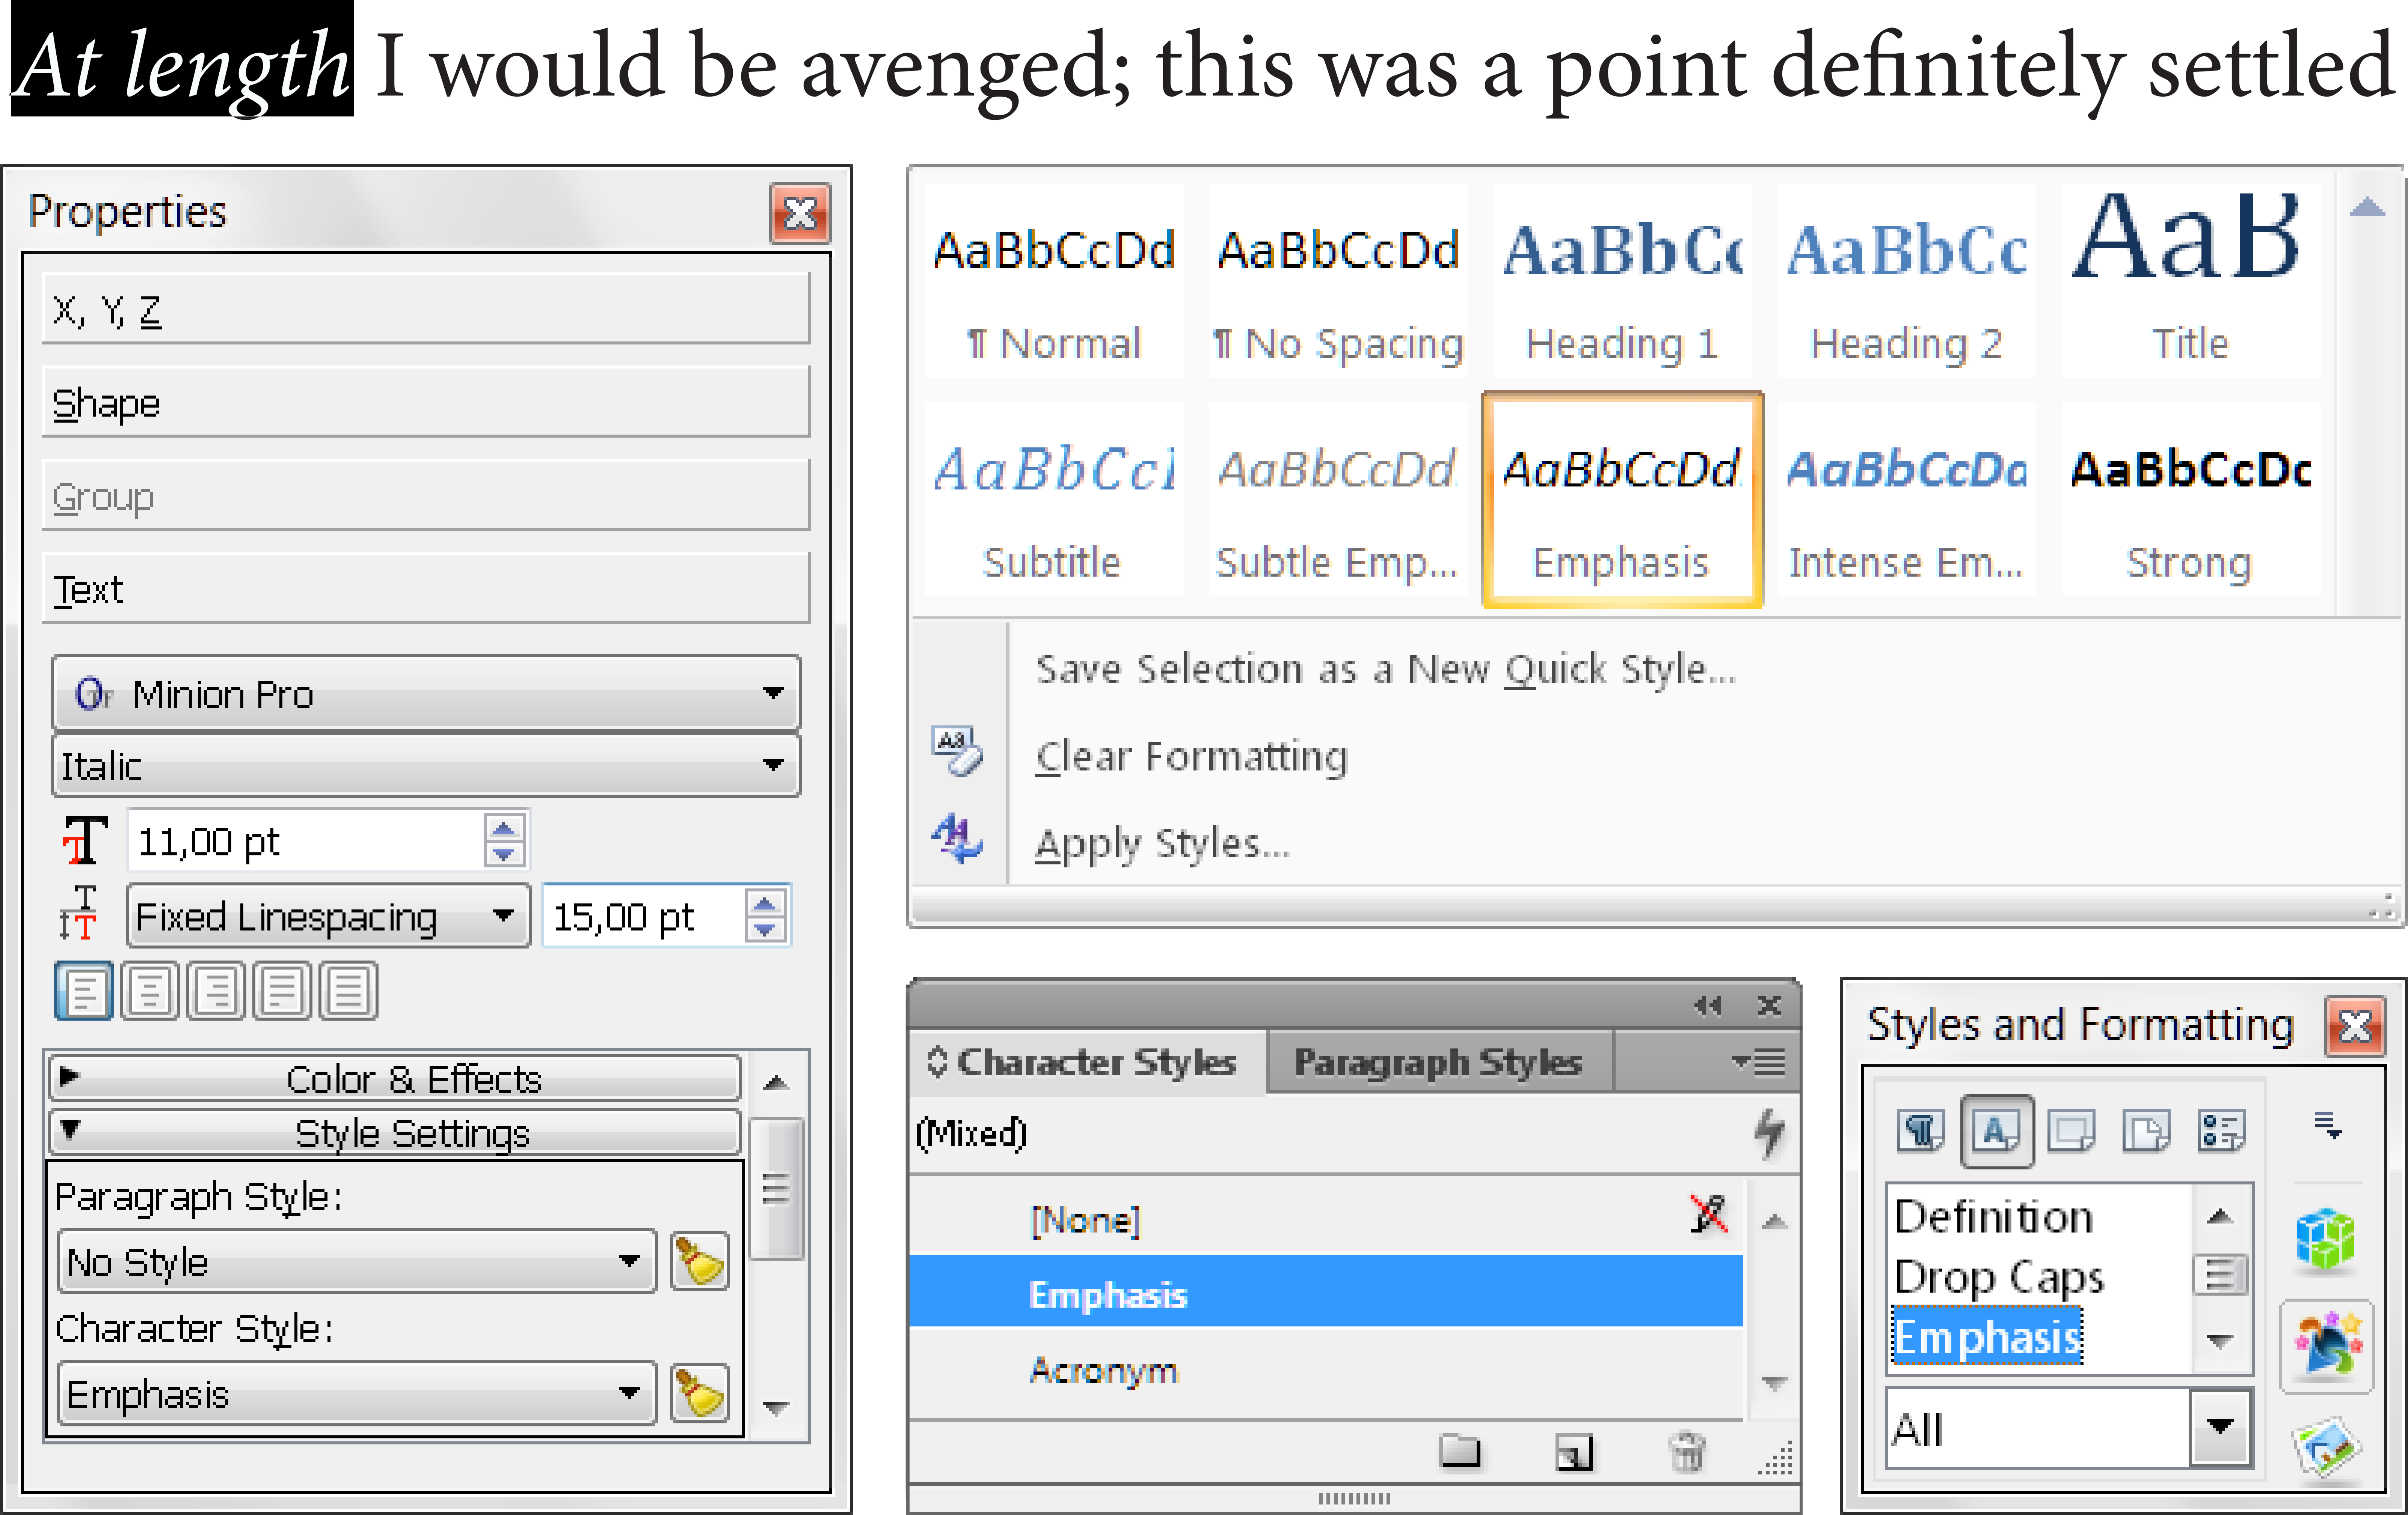
\includegraphics[width=\textwidth]{examples/02/interactive-editors.png}
  \caption{Logical markup in the interactive \acropl{DPS} of \inx{Scribus}
    (left), \inx{Microsoft Word} (top), \inx{Adobe InDesign} (bottom left) and
    \inx{Apache OpenOffice} (bottom right)}
\end{figure}

\section{Lightweight Markup Languages}
Parallel to the heavy-duty applications of \acronym{SGML} and \acronym{XML},
there runs a vein of markup languages that give priority to unobtrusiveness and
legibility over raw expressive power. Rooted in the reality of computer text
terminals with limited formatting capabilities, \termpl{lightweight markup
language} leverage punctuation and indentation to produce comparatively weak and
domain-specific, but also humane, highly intuitive, and often profoundly
beautiful markup that is easy to both read and write. Examples of lightweight
markup languages include \inx{Markdown}, \inx{Creole}, \inx{AsciiDoc},
\inx{MakeDoc}, \inx{Setext}, and \inx{Wikicode}.  Lightweight markup languages
are typically supplemented by tools that enable the conversion to more general
markup languages, such as \acronym{HTML}. The more popular lightweight markup
languages come in various flavors that represent their use cases.
